\documentclass[a4paper,11pt]{article}

\usepackage[T1]{polski}
\usepackage[utf8]{inputenc} 
\usepackage{graphicx}
\usepackage{float}
\usepackage{verbatim}
\hoffset=-3.0cm                 % Mniejszy lewy margines
\textwidth=18cm                 % szerzej
\evensidemargin=0pt

\voffset=-3cm                   % Mniejszy gorny margines
\textheight=27cm                % szerzej wzdluz

\usepackage{listings}
% Listingi
\lstdefinestyle{customc}{
	belowcaptionskip=1\baselineskip,
	breaklines=true,
	frame=L,
	xleftmargin=0pt,
	language=HTML,
	showstringspaces=false,
	basicstyle=\footnotesize\ttfamily,
	identifierstyle=\color{black}
}

\setlength{\parindent}{0pt}             % No paragraph indentation
\setlength{\parskip}{\medskipamount}    % Space between paragraphs
\raggedbottom   


\title{POLITECHNIKA WARSZAWSKA \\ WYDZIAŁ ELEKTRYCZNY \\}
\author{Michał Sut}
\date{\today}

\begin{document}
	\thispagestyle{empty}
	\maketitle
	\date{}
	\section{Treść zadania}
	Napisać program umożliwiający znalezienie maksimum funkcji dopasowania jednej 
	zmiennej określonej dla liczb całkowitych w zadanym zakresie przy pomocy 
	elementarnego algorytmu genetycznego (reprodukcja z użyciem nieproporcjonalnej 
	ruletki, krzyżowanie proste, mutacja równomierna). Program powinien umożliwiać 
	użycie różnych funkcji dopasowania, populacji o różnej liczebności oraz różnych 
	parametrów operacji genetycznych (krzyżowania i mutacji). Program powinien 
	zapewnić wizualizację wyników w postaci wykresów średniego, maksymalnego 
	i minimalnego przystosowania dla kolejnych populacji oraz wykresu funkcji 
	w zadanym przedziale. 
	
	Program przetestować dla funkcji$ f(x)= -0.1x^2 + 4x + 7 $ dla $x= -1, 0, ... 41 $

	\section{Instrukcja działania programu}
		\subsection{Uruchomienie}
			Program został napisany w języku Python, z wykorzystaniem bibliotek zawartych w dystrybucji Anaconda3. W związku z tym, należy uruchamiać program w tym środowisku, z linii poleceń. Aby uruchomić program należy wpisać w konsoli:\\~\\
			\texttt{\$ python ag.py} 
		\subsection{Okno główne programu}
			\begin{figure}[H]
				\centering
				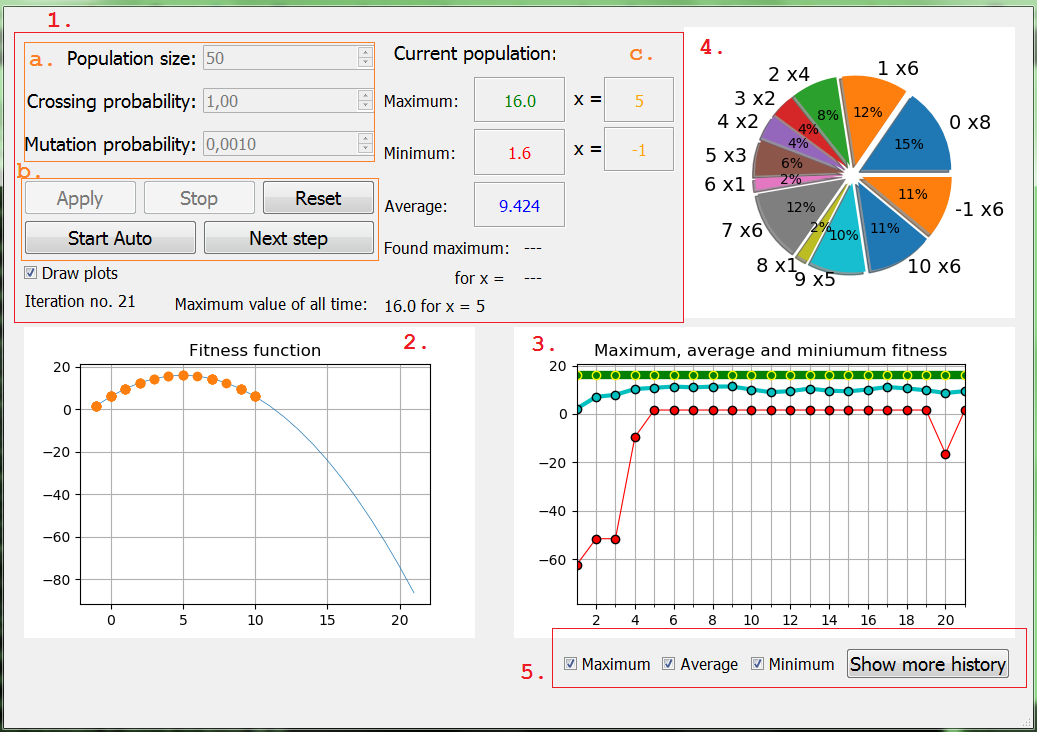
\includegraphics[scale=0.6]{main_window2.png}
			\end{figure}
		
		\subsection{Opis okna programu}
			\begin{enumerate}
				\item Panel sterowania
				\begin{enumerate}
					\item Parametry populacji
					\item Przyciski sterowania
					\item Wszystkie informacje gromadzone i wyliczone podczas działania programu
				\end{enumerate}
				\item Wykres funkcji z zaznaczonymi osobnikami populacji
				\item Wykres wartości średnich, maksymalnych i minimalnych dla kolejnych generacji. Pokazuje określoną liczbę ostatnich wyników. 
				\item Wykres kołowy przedstawiający "nieproporcjonalną ruletkę", czyli prawdopodobieństwo wylosowania danego osobnika
				\item Panel umożliwiający podejrzenie całego wykresu, aż od początkowej generacji.
			\end{enumerate}
		
		\subsection{Zmiana ustawień programu}
			Ustawienia programu znajdują się w pliku \texttt{settings.py}. Zmianą podlegają następujące elementy:
			\begin{enumerate}
				\item \textbf{FUNCTION} - Funkcja dopasowania
				\item \textbf{X\_START} - Początek zakresu
				\item \textbf{X\_END} - Koniec zakresu
				\item \textbf{MAX\_HIST\_SIZE} - Liczba wyników pokazywana na wykresie wartości min/max/avg
			\end{enumerate}
	
		\subsection{Użycie}
			\subsubsection{Podstawowe operacje}
				\begin{enumerate}
					\item Ustawić parametry populacji
					\item Zainicjować populację klikając przycisk \framebox{ \texttt{Apply}}
					\item W tym momencie dostępne są trzy możliwości:
					\begin{enumerate}
						\item \framebox{Next Step} - Wykonanie tylko jednej generacji
						\item \framebox{Start Auto} - Wykonywanie kolejnych generacji aż do wystąpienia warunku stopu
						\item \framebox{Reset} - Wyczyszczenie populacji i jej parametrów
					\end{enumerate}
					\item Rozpoczęty proces automatycznych generacji można zastopować przyciskiem \framebox{Stop}
				\end{enumerate}
				
				Zaznaczając lub odznaczając pole \texttt{Draw plots} decydujemy o tym, czy kolejne generacje będą wyświetlane na wykresach.\\
				\emph{Uwaga! Zaznaczenie pola powoduje wydłużenie czasu trwania wykonania jednego pełnego kroku. Ma to szczególne znaczenie podczas generacji automatycznych.}
			\subsubsection{Otworzenie pełnego wykresu wartości średnich, maksymalnych i minimalnych}
			Przycisk \framebox{Show more history} powoduje otworzenie nowego okna z pełnym wykresem wartości, które zostały zaznaczone w polach, znajdujących się obok przycisku. Nowo otwarte okno wygląda następująco: 
			\begin{figure}[H]
				\centering
				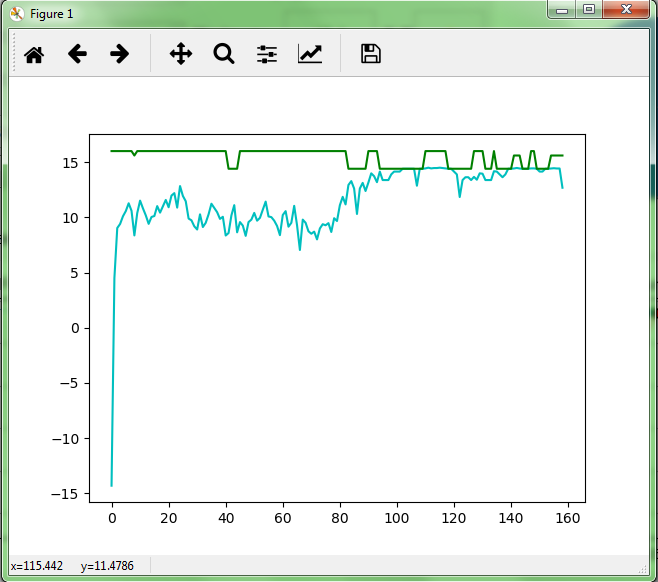
\includegraphics[scale=0.8]{full_plot.png}
			\end{figure}
				
			Możemy przybliżać i oddalać dowolne fragmenty wykresu, modyfikować wygląd wykresu, a także zapisać go do pliku \texttt{*.png}
			
		\subsection{Warunek stopu}
		Program powinien zatrzymać się po wykonaniu przynajmniej 1000 iteracji, w sytuacji gdy ostanie 20 wartości maksymalnych jest takich samych, a w populacji występują tylko osobniki o tym samym kodzie.
		
	\section{Opis eksperymentów}
	Eksperymenty przeprowadzone były dla funkcji $f(x) = -0.1x^2 + 4x + 7$, dla $x = -1, 0, ..., 41$. Dokładność znalezionego rozwiązania obliczona jest poprzez obliczenie stosunku znalezionej wartości maksymalnej do wartości obliczonej analitycznie. W tym przypadku, maksimum funkcji wynosi $47$ i jest osiągane dla argumentu $x = 20$
	
		\subsection{Różna liczebność populacji}
			W celu przeprowadzenia tych eksperymentów, kilkukrotnie uruchomione zostanie  automatyczne znajdowanie maksimum dla populacji z domyślnymi parametrami prawdopodobieństwa mutacji (0,001) i krzyżowania (1,00).
			\subsubsection{Populacja: 4 osobników}
				Wyniki prezentują się następująco:\\~\\
				\begin{tabular}{|c|c|c|c|c|c|}
					\hline 
					Lp & X & maksimum & Błąd X & Błąd maks & Liczba iteracji\\
					\hline
					1 & 21  & 46,9 & 5,00\%  & 0,21\% & 1001\\\hline
					2 & 19 & 46,9  & 5,00\% & 0,21\% & 1002\\\hline
					3 & 20  & 47   & 0,00\%  & 0,00\% & 1001\\\hline
					4 & 26 & 43,4  & 30,00\%  & 7,66\% & 1003\\\hline
					5 & 31 & 34,9  & 55,00\%  & 25,74\% & 1001\\\hline
					6 & 15 & 44,5  & 25,00\%  & 5,32\% & 1001\\\hline
					8 & 14 & 43,4  & 30,00\%  & 7,66\% & 1009\\\hline
					9 & 18 & 46,6  &  10,00\% & 0,85\% & 1001\\\hline
					10 & 14 & 43,4 & 30,00\% & 7,66\%& 1001\\\hline
				\end{tabular} 
			\subsubsection{Populacja: 10 osobników}
				Wyniki prezentują się następująco:\\~\\
				\begin{tabular}{|c|c|c|c|c|c|}
					\hline 
					Lp & X & maksimum & Błąd X & Błąd maks. & Liczba iteracji\\\hline
					1 & 21 & 46,9 & 5,00\% &0,21\%  &1001\\\hline
					2 & 23 & 46,1 & 15,00\% & 1,91\% &1001 \\\hline
					3 & 22 & 46,6 & 10,00\% &0,85\% &1002 \\\hline
					4 & 19 & 46,9 & 5,00\% & 0,21\%&1040 \\\hline
					5 & 18 & 46,6 & 10,00\% & 0,85\%&1021 \\\hline
					6 & 20 & 47,0 & 0,00\% & 0,00\%& 1032 \\\hline
					8 & 26 & 43,4 & 30,00\% & 7,66\%& 1022 \\\hline
					9 & 23 & 46,1 & 15,00\% & 1,91\%& 1001 \\\hline
					10 & 17 & 46,1&15,00\%  & 1,91\%& 1004 \\\hline
				\end{tabular} 
			\subsubsection{Populacja: 50 osobników}
				Wyniki prezentują się następująco:\\~\\
				\begin{tabular}{|c|c|c|c|c|c|}
					\hline 
					Lp & X & maksimum & Błąd X & Błąd maks. & Liczba iteracji \\
					\hline
					1 & 23 & 46,1 & 15,00\% & 1,91\%& 1008\\\hline
					2 & 19 & 46,9 & 5,00\% & 0,21\%& 1017\\\hline
					3 & 23 & 46,1 & 15,00\% & 1,91\% & 1021 \\\hline
					4 & 21 & 46,9 & 5,00\% & 0,21\% & 1100\\\hline
					5 & 19 & 46,9 & 5,00\% & 0,21\% & 1033\\\hline
					6 & 21 & 46,9 & 5,00\% & 0,21\% & 1152\\\hline
					8 & 20 & 47,0 & 0,00\% & 0,00\% & 1001\\\hline
					9 & 23 & 46,1 & 15,00\% &1,91\%  & 1009\\\hline
					10& 20 & 47,0 & 0,00\% & 0,00\% & 1156 \\\hline
				\end{tabular} 
			\subsubsection{Populacja: 100 osobników}
				Wyniki prezentują się następująco:\\~\\
				\begin{tabular}{|c|c|c|c|c|c|}
					\hline 
					Lp & X & maksimum & Błąd X & Błąd maks. & Liczba iteracji\\
					\hline
					1 & 19 & 46,9 & 5,00\% & 0,21\% & 1452\\\hline
					2 & 21  & 46,9 & 5,00\% & 0,21\% & 1092 \\\hline
					3 & 20 & 47,0 & 0,00\% & 0,00\% & 1065\\\hline
					4 & 18 & 46,6 & 10,00\% & 0,85\% & 1001 \\\hline
					5 & 23 & 46,1 & 15,00\% & 1,91\% & 1028 \\\hline
					6 & 18 & 46,6 & 10,00\% & 0,85\% & 1475\\\hline
					8 & 21 & 46,9 & 5,00\% & 0,21\% & 1101\\\hline
					9 & 20 & 47,0 & 0,00\% & 0,00\% & 1503\\\hline
					10 & 21 & 46,9 & 5,00\% & 0,21\% & 1124\\\hline
				\end{tabular} 
			\subsection{Różne prawdopodobieństwa krzyżowania}
				Eksperymenty przeprowadzone będą dla populacji 10 osobników, z prawdopodobieństwem mutacji równym 0.001
				\subsubsection{Krzyżowanie: prawdopodobieństwo = 1,00}
					Wyniki prezentują się następująco:\\~\\
					\begin{tabular}{|c|c|c|c|c|c|}
						\hline 
						Lp & X & maksimum & Błąd X & Błąd maks. & Liczba iteracji\\\hline
						1 & 21 & 46,9 & 5,00\% &0,21\%  &1001\\\hline
						2 & 23 & 46,1 & 15,00\% & 1,91\% &1001 \\\hline
						3 & 22 & 46,6 & 10,00\% &0,85\% &1002 \\\hline
						4 & 19 & 46,9 & 5,00\% & 0,21\%&1040 \\\hline
						5 & 18 & 46,6 & 10,00\% & 0,85\%&1021 \\\hline
						6 & 20 & 47,0 & 0,00\% & 0,00\%& 1032 \\\hline
						8 & 26 & 43,4 & 30,00\% & 7,66\%& 1022 \\\hline
						9 & 23 & 46,1 & 15,00\% & 1,91\%& 1001 \\\hline
						10 & 17 & 46,1&15,00\%  & 1,91\%& 1004 \\\hline
					\end{tabular} 
				\subsubsection{Krzyżowanie: prawdopodobieństwo = 0,90}
					Wyniki prezentują się następująco:\\~\\
					\begin{tabular}{|c|c|c|c|c|c|}
						\hline 
						Lp & X & maksimum & Błąd X & Błąd maks &Liczba iteracji\\
						\hline
						1 & 22 & 46,1 & 10,00\% &1,91\% & 1016 \\\hline
						2 & 16 & 45,4 & 20,00\% &3,40\% & 1146  \\\hline
						3 & 25 & 44,5 & 25,00\% &5,32\% &1043 \\\hline
						4 & 25 & 44,5 & 25,00\% &5,32\% &1001 \\\hline
						5 & 16 & 45,4 & 20,00\% &3,40\% &1057 \\\hline
						6 & 14 & 43,4 & 30,00\% &7,66\% &1001 \\\hline
						8 & 23 & 46,1 & 15,00\% &1,91\% &1001 \\\hline
						9 & 25 & 44,5 & 25,00\% &5,32\% &1001 \\\hline
						10& 16 & 45,4 & 20,00\% &3,40\%&1001 \\\hline
					\end{tabular}
				\subsubsection{Krzyżowanie: prawdopodobieństwo = 0,50}
					Wyniki prezentują się następująco:\\~\\
					\begin{tabular}{|c|c|c|c|c|c|}
						\hline 
						Lp & X & maksimum & Błąd X & Błąd maks. & Liczba iteracji\\
						\hline
						1 & 11 & 38,9 & 45,00\% &17,23\% &1001 \\\hline
						2 & 20 & 47,0 & 0,00\% &0,00\% &1001  \\\hline
						3 & 19 & 46,9 & 5,00\% & 0,21\%&1001 \\\hline
						4 & 25 & 44,5 & 25,00\% &5,32\% &1003 \\\hline
						5 & 21 & 46,9 & 5,00\% & 0,21\%&1001 \\\hline
						6 & 14 & 43,4 & 30,00\% & 7,66\%&1001 \\\hline
						8 & 23 & 46,1 & 15,00\% & 1,91\%&1001 \\\hline
						9 & 15 & 44,5 & 25,00\% & 5,32\%&1001 \\\hline
						10& 21 & 46,9 & 5,00\% &0,21\% &1001 \\\hline
					\end{tabular} 
				\subsubsection{Krzyżowanie: prawdopodobieństwo = 0,00}
					Wyniki prezentują się następująco:\\~\\
					\begin{tabular}{|c|c|c|c|c|c|}
						\hline 
						Lp & X & maksimum & Błąd X & Błąd maks. & Liczba iteracji\\
						\hline
						1 & 11 & 38,9 & 45,00\% & 17,23\% & 1001 \\\hline
						2 & 19 & 46,9 & 5,00\% & 0,21\%& 1039 \\\hline
						3 & 25 & 44,5 & 25,00\% &5,32\% &1001 \\\hline
						4 & 19 & 46,9 & 5,00\% &0,21\% &1001 \\\hline
						5 & 21 & 46,9 & 5,00\% &0,21\% &1001 \\\hline
						6 & 24 & 45,4 & 20,00\% &3,40\% &1002 \\\hline
						8 & 21 & 46,9 & 5,00\% &0,21\% &1001 \\\hline
						9 & 15 & 44,5 & 25,00\% & 5,32\%&1001 \\\hline
						10 & 20 & 47,0 & 0,00\% & 0,00\%&1003 \\\hline
					\end{tabular} 
			\subsection{Różne prawdopodobieństwa mutacji}
				Eksperymenty przeprowadzone będą dla populacji 10 osobników, z prawdopodobieństwem krzyżowania równym 1,00
				\subsubsection{Mutacja: prawdopodobieństwo = 0,000}
					Wyniki prezentują się następująco:\\~\\
					\begin{tabular}{|c|c|c|c|c|c|}
						\hline 
						Lp & X & maksimum & Błąd X & Błąd maks. & Liczba iteracji\\
						\hline
						1 & 10 & 37,0 & 50,00\% &21,28\% &1001 \\\hline
						2 & 27 & 42,1 & 35,00\% &10,43\% &1001 \\\hline
						3 & 15 & 44,5 & 25,00\% &5,32\% &1001 \\\hline
						4 & 12 & 40,6 & 40,00\% &13,62\% &1001 \\\hline
						5 & 10 & 37,0 & 50,00\% &21,28\% &1001 \\\hline
						6 & 25 & 44,5 & 25,00\% &5,32\% &1001 \\\hline
						8 & 25 & 44,5 & 25,00\% & 5,32\%&1001 \\\hline
						9 & 15 & 44,5 & 25,00\% & 5,32\%&1001 \\\hline
						10 & 30 & 37,0 & 50,00\% & 21,28\%&1001 \\\hline
					\end{tabular} 
				\subsubsection{Mutacja: prawdopodobieństwo = 0,001}
					Wyniki prezentują się następująco:\\~\\
					\begin{tabular}{|c|c|c|c|c|c|}
						\hline 
						Lp & X & maksimum & Bład X & Bład max & Liczba iteracji\\\hline
						1 & 21 & 46,9 & 5,00\% &0,21\%  &1001\\\hline
						2 & 23 & 46,1 & 15,00\% & 1,91\% &1001 \\\hline
						3 & 22 & 46,6 & 10,00\% &0,85\% &1002 \\\hline
						4 & 19 & 46,9 & 5,00\% & 0,21\%&1040 \\\hline
						5 & 18 & 46,6 & 10,00\% & 0,85\%&1021 \\\hline
						6 & 20 & 47,0 & 0,00\% & 0,00\%& 1032 \\\hline
						8 & 26 & 43,4 & 30,00\% & 7,66\%& 1022 \\\hline
						9 & 23 & 46,1 & 15,00\% & 1,91\%& 1001 \\\hline
						10 & 17 & 46,1&15,00\%  & 1,91\%& 1004 \\\hline
					\end{tabular} 
				\subsubsection{Mutacja: prawdopodobieństwo = 0,004}
					Wyniki prezentują się następująco:\\~\\
					\begin{tabular}{|c|c|c|c|c|c|}
						\hline 
						Lp & X & maksimum & Błąd X & Błąd maks. & Liczba iteracji\\
						\hline
						1 & 21 & 46,9 & 5,00\%  & 0,21\%  &1001\\\hline
						2 & 18 & 46,6 & 10,00\% & 0,85\% & 1052\\\hline
						3 & 23 & 46,1 & 15,00\% & 1,91\% &1001\\\hline
						4 & 21 & 46,9 & 5,00\%  & 0,21\% &1001\\\hline
						5 & 17 & 46,1 &  15,00\%& 1,91\% &1116\\\hline
						6 & 21  & 46,9 & 5,00\% & 0,21\% &1122\\\hline
						8 & 18 & 46,6 & 10,00\% & 0,85\% &1003\\\hline
						9 & 23 & 46,1 & 15,00\% & 1,91\% &1029\\\hline
						10 & 20 & 47,0 & 0,00\% & 0,00\% &1001\\\hline
					\end{tabular} 
			\subsection{Podsumowanie eksperymentów}
			\begin{tabular}{|c|c|c|}
				\hline
				Eksperyment & średnie maksimum & odchylenie stand. średniej maks. \\\hline
				Populacja: 4  & 44,10 & 3,80\\\hline
				Populacja: 10 &46,20 &1,10 \\\hline
				Populacja: 50 & 46,66& 0,42\\\hline
				Populacja: 100&46,77 &0,29\\\hline
				Krzyżowanie: 1,00& 46,20 & 1,10 \\\hline
				Krzyżowanie: 0,09& 45,03 & 0,88 \\\hline
				Krzyżowanie: 0,05& 45,011 &2,65 \\\hline
				Krzyżowanie: 0,00&  45,322 & 2,63\\\hline
				Mutacja: 0,000& 41,3 & 3,49\\\hline
				Mutacja: 0,001& 46,20 & 1,10\\\hline
				Mutacja: 0,004& 46,58& 0,38 \\\hline
			\end{tabular}
	\section{Wnioski}
		Przeprowadzone eksperymenty pokazują, że zmiana parametrów populacji wpływa na znajdowanie maksimum funkcji dopasowania danej populacji. 
		\subsection{Wniosek 1. Dokładność algorytmu}
		Algorytm nie zawsze znajduje wartość maksymalną. W większości przypadków znajdowane były wartości bliskie oczekiwanej, czyli osobniki, o kodzie zbliżonym to najlepszego. Wynika to z faktu, iż funkcja dopasowania, dla której przeprowadzone były eksperymenty zwraca zbliżone wartości dla osobników o kodzie bliskim najlepszego. Na fakt znalezienia lub nie znalezienia realnej wartości maksymalnej wpływają parametry populacji.
		\subsection{Wniosek 2. Wpływ liczby osobników w populacji na wynik działania algorytmu}
		Przeprowadzone eksperymenty pokazują, że statystycznie lepsze wyniki uzyskiwane są dla większych populacji. Największa z badanych przeze mnie populacji dała najwyższy średni wynik z 10 prób, co oznacza najmniejszy błąd względem wartości wyliczonej analitycznie.\\ Dodatkowo, można stwierdzić, że dla większych populacji wyniki są bardziej jednorodne i skupiają się wokół realnej wartości maksymalnej. Wynika to z faktu, iż najliczebniejsza z badanych populacji zwracała wyniki, których odchylenie standardowe było najmniejsze. \\
		Jednakże, im większa populacja, tym więcej iteracji algorytmu jest potrzebne, aby wystąpił warunek stopu i znaleziona została wartość maksymalna.
		\subsection{Wniosek 3. Wpływ prawdopodobieństwa krzyżowania na wynik działania algorytmu}
		Krzyżowanie, jak każdy z parametrów, wpływa na dokładność wyniku, lecz jego wpływ w przeprowadzonym badaniu, nie był tak bardzo widoczny jak wpływ liczebności populacji.\\
		Zmniejszenie prawdopodobieństwa krzyżowania powoduje, że znalezione wartości są bardziej zróżnicowane, czyli odchylenie standardowe wyników wzrasta. \\
		Wykonany eksperyment pokazał, że gdy krzyżowanie jest pewne, średni wynik jest lepszy. Mniejsze wartości powoduję wyniki średnio niższe, jednak nie można stwierdzić, że wynik jest proporcjonalny do prawdopodobieństwa krzyżowania. \\
		Wpływ krzyżowania najbardziej widać w sytuacji, gdy w populacji startowej, nie ma osobników o najlepszym dopasowaniu lub zbliżonych do nich. Wyniki wtedy są gorsze, ponieważ tworzy się mniej nowych potencjalnych rozwiązań. 
		Co więcej, mniejsza szansa na krzyżowanie powoduje mniejszą wymaganą liczbę iteracji do zakończenia wykonywaniu algorytmu
		\subsection{Wniosek 3. Wpływ prawdopodobieństwa mutacji na wynik działania algorytmu}
		Eksperyment pokazał, że zwiększenie szansy na mutacje, zwiększa prawdopodobieństwo znalezienia maksimum oraz zwiększa średni wynik z kilku prób. Dodatkowo, zróżnicowanie wyników jest mniejsze dla większej wartości prawdopodobieństwa mutacji. Spowodowane jest to tym, że mutacje znacznie zwiększają liczbę potencjalnych rozwiązań.\\
		Zwiększenie tego parametru ma także negatywny skutek. Liczba iteracji potrzebna do zakończenia algorytmu dla populacji, w której mutacje występują częściej jest większa.
		
	
\end{document}